% !TEX encoding = UTF-8 Unicode
% !TEX root = ../Rapport/rapport.tex

\section{Comparaison de \emph{branch and bound} et \emph{branch and cut}}

Nous considérons le  programme linéaire suivant :
$$
PL_0 \begin{cases}
max\ z(x_1,x_2) = 2x_1 + x_2 \\
 2x_1 + 5x_2 \leq 17 \\
 3x_1 + 2x_2 \leq 10 \\
 x_1, x_2 \geq 0 \\
\end{cases}
$$

\subsection{Polytope associé à ${PL}_0$}
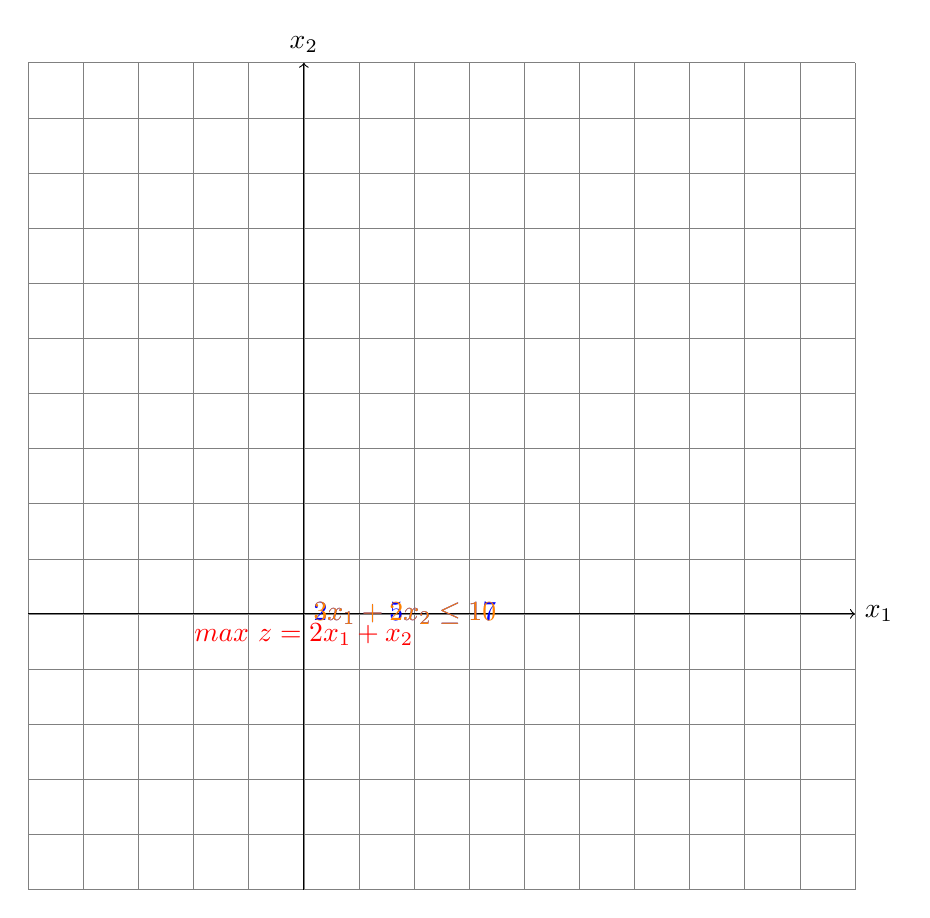
\begin{tikzpicture}[scale = 0.7]
    \draw[very thin,color=gray] (-5,-5) grid (10, 10);
    \draw[->] (-5,0) -- (10,0) node[right] {$x_1$};
    \draw[->] (0,-5) -- (0,10) node[above] {$x_2$};
    \draw[color=red, domain=-5:2.5] plot[id=obj] function{-2*x} 
        node[below] {$max\ z = 2x_1 + x_2$};
    \draw[color=blue, domain=-5:10] plot[id=c1] function{(17.0/5.0) - (3.0/5.0)*x} 
        node[right] {$2x_1 + 5x_2 \leq 17$};
    \draw[color=orange, domain=-10.0/3.0:20.0/3.0] plot[id=c2] function{(5.0)-(3.0/2.0)*x)} 
        node[right] {$3x_1+2x_2 \leq 10$};
\end{tikzpicture}


\subsection{Résolution graphique}
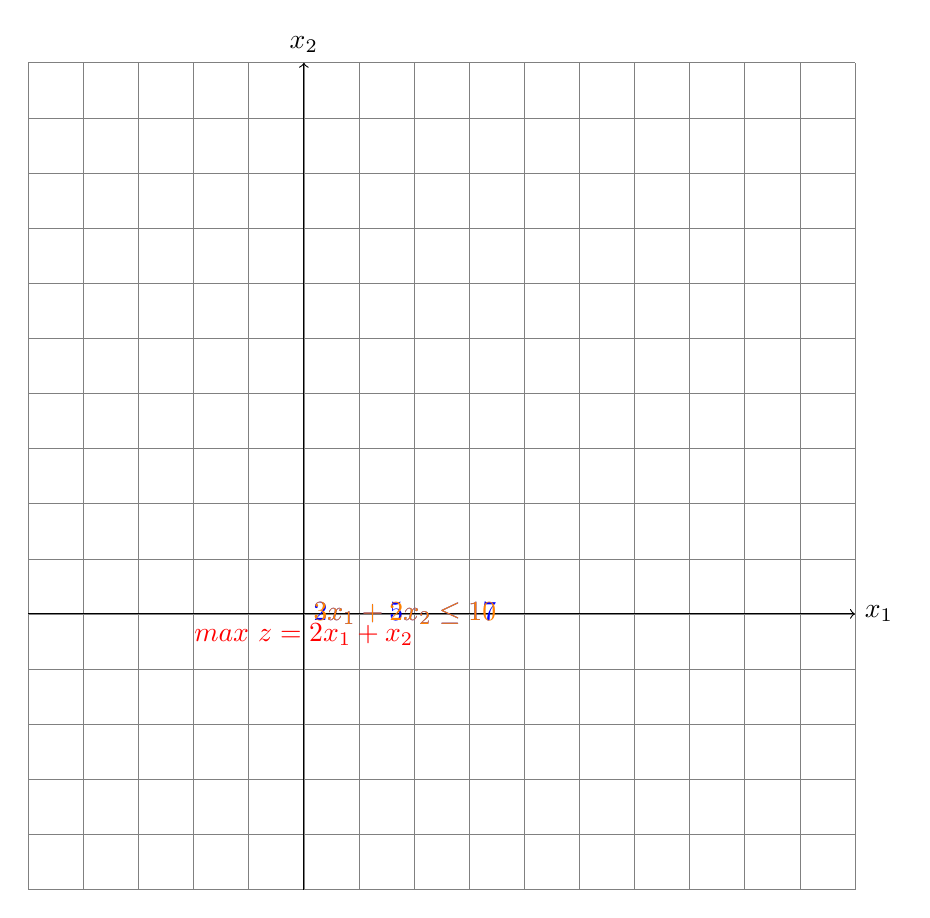
\begin{tikzpicture}[scale = 0.7]
    \draw[very thin,color=gray] (-5,-5) grid (10, 10);
    \draw[->] (-5,0) -- (10,0) node[right] {$x_1$};
    \draw[->] (0,-5) -- (0,10) node[above] {$x_2$};
    \draw[color=red, domain=-2:6] plot[id=obj] function{6.6-2*x} 
        node[below] {$max\ z = 2x_1 + x_2$};
    \draw[color=blue, domain=-5:10] plot[id=c1] function{(17.0/5.0) - (3.0/5.0)*x} 
        node[right] {$2x_1 + 5x_2 \leq 17$};
    \draw[color=orange, domain=-10.0/3.0:20.0/3.0] plot[id=c2] function{(5.0)-(3.0/2.0)*x)} 
        node[right] {$3x_1+2x_2 \leq 10$};
\end{tikzpicture}


\subsection{Résolution par la méthode du simplexe}


\subsection{Recherche d'une solution à valeurs entières}

\subsubsection{Branch and bound}

\subsubsection{Coupes de Gomory}